\documentclass{beamer}
\usetheme{Madrid}
% Use a neutral colortheme so we can fully override colors
\usecolortheme{default}
\usepackage{minted}

% use tikz for generating diagrams
\usepackage{tikz}
\usetikzlibrary{arrows.meta,calc,angles,quotes,positioning}

% for links
\usepackage{hyperref}

% UPenn color palette
\definecolor{PennBlue}{RGB}{1,31,91}   % #011F5B
\definecolor{PennRed}{RGB}{153,0,0}    % #990000

% Apply colors to beamer elements
\setbeamercolor{structure}{fg=PennBlue}
% Make title slide text white for contrast on dark background
\setbeamercolor{title}{fg=white}
\setbeamercolor{subtitle}{fg=black}
\setbeamercolor{author}{fg=black}
\setbeamercolor{date}{fg=black}
% Ensure the title page itself uses our dark background and white foreground
\setbeamercolor{title page}{bg=PennBlue,fg=black}
\setbeamercolor{frametitle}{fg=white,bg=PennBlue}
\setbeamercolor{normal text}{fg=black,bg=white}

% Headline/footline palettes (Madrid uses these)
\setbeamercolor{palette primary}{bg=PennBlue, fg=white}
\setbeamercolor{palette secondary}{bg=PennRed,  fg=white}
\setbeamercolor{palette tertiary}{bg=PennBlue!80!black, fg=white}
\setbeamercolor{palette quaternary}{bg=PennRed!80!black,  fg=white}

% Blocks and emphasis
\setbeamercolor{block title}{fg=white,bg=PennBlue}
\setbeamercolor{block body}{bg=PennBlue!5}
\setbeamercolor{alerted text}{fg=PennRed}
\setbeamercolor{example text}{fg=PennBlue}
\setbeamercolor{itemize item}{fg=PennBlue}
\setbeamercolor{itemize subitem}{fg=PennRed}

% Footer styling colors
\setbeamercolor{author in head/foot}{bg=PennBlue,fg=white}
\setbeamercolor{title in head/foot}{bg=PennRed,fg=white}
\setbeamercolor{date in head/foot}{bg=PennBlue,fg=white}

% Custom footline with course and term centered
\setbeamertemplate{footline}{
  \leavevmode
  \hbox{%%
    \begin{beamercolorbox}[wd=.33\paperwidth,ht=2.5ex,dp=1ex,left]{author in head/foot}
      \hspace{1em}\insertshortauthor
    \end{beamercolorbox}%%
    \begin{beamercolorbox}[wd=.34\paperwidth,ht=2.5ex,dp=1ex,center]{title in head/foot}
      Lecture 12
    \end{beamercolorbox}%%
    \begin{beamercolorbox}[wd=.33\paperwidth,ht=2.5ex,dp=1ex,right]{date in head/foot}
      \insertframenumber{} / \inserttotalframenumber\hspace{1em}
    \end{beamercolorbox}%%
  }
  \vskip0pt
}

% Remove navigation symbols
\setbeamertemplate{navigation symbols}{}


\title{Lecture 13}
\author{ENGR1050 Fall 2025}
\date{\today}

\begin{document}

% Title frame with UPenn logo

\begin{frame}
  \vfill
  \begin{center}

    % Title and course info
    {\Large\textbf{ENGR1050: Lecture 13}}
    \vskip1em
    {\large Differential equations and numerical methods}
    \vskip0.5em
    {\insertdate}
    \vskip2em
    % UPenn logo at bottom
    \includegraphics[height=2.5cm]{upennlogo.png}

  \end{center}
  \vfill
\end{frame}

\begin{frame}{Agenda}
  \begin{itemize}
    \item Last class we built a class for solving ODEs numerically together
    \item Today we'll get some extra practice using it to model a pendulum
    \item We have lab this Wednesday (\textbf{meet in GM lab}) where we will use \textit{potentiometers} to measure angles of pendulums
  \end{itemize}
  \textit{Important note:} Prof. Trask is on travel Tuesday so can't make OH; today's exercise should get you the help you need to finish the homework or you can meet with Ben. HW is pushed back to Thursday.
\end{frame}

  \begin{frame}{Numerical solution of ODEs}
    Many ODEs cannot be solved analytically, so we use numerical methods to approximate solutions. The simplest is the Explicit Euler method.
  \begin{definition}
    For the IVP \(y'(t)=f(t,y)\) with \(y(t_0)=y_0\) and step size \(h>0\), the Starting from $t_0,y_0$, Explicit Euler scheme updates via
    \[
      t_{n+1}=t_n+h, \qquad
      y_{n+1}=y_n + h\,f(t_n,y_n),
    \]
  \end{definition}
  \begin{figure}
    \centering
    \includegraphics[width=0.4\textwidth]{expliciteuler.jpg}
    \caption{Graphical representation of the Explicit Euler method. The tangent line at each point is used to estimate the next point.}
  \end{figure}
\end{frame}

  \begin{frame}[fragile]{Last lecture's ODE\_solver class}
    \begin{minted}[fontsize=\tiny,breaklines=true]{python}
class ODE_solver:
    def __init__(self, t0, tf, y0, N):
        self.y0 = y0  # initial condition as numpy array
        self.t0 = t0  # initial time as float
        self.tf = tf  # final time as float
        self.N = N    # number of steps as integer
        self.h = (tf - t0) / float(N) # timestep size

        # We need to check what size y0 is and store that information
        self.dim = len(y0) #assumes that y0 is a list or array

        # Create a place to store the solution
        self.t_values = np.array([t0 + i*self.h for i in range(N+1)])  # time values
        self.solution = np.zeros((N+1, self.dim))  # solution array
        self.solution[0, :] = y0  # set initial condition
        
    def f(self,t,y):
        # Define the right-hand side of the ODE here, assuming a scalar t and a numpy array y
        # Example: dy/dt = -2y (for scalar y),
        # this function should return a numpy array of the same shape as y
        f = np.zeros_like(y)
        f[0] = -2 * y[0]  # Example for the first component
        return f
    
    def solve(self):
        # Implement explicit euler: y_n+1 = y_n + h*f(t_n, y_n)
        for n in range(self.N):
            t_n = self.t_values[n]
            y_n = self.solution[n, :]
            f_n = self.f(t_n, y_n)
            self.solution[n+1, :] = y_n + self.h * f_n
        return self.solution
    \end{minted}
\end{frame}

\begin{frame}{We discussed: best practices for solving an ODE.}
  \begin{itemize}
    \item Implement the RHS of the ODE in the \textit{f} method
    \item Instantiate the class with initial conditions, final time, and number of steps
    \item Call the \textit{solve()} method to compute the numerical solution
    \item \textbf{Convergence study:} Increase $N$ and run again by re-instantiating the class; repeat until solution doesn't change
    \item \textbf{Validation:} Compare to analytical solution or asymptotic behavior
  \end{itemize}
  The homework consists of solving two different numerical ODEs with this code. We will work through an example today that should help you finish the homework and also prepare you for Wednesday's lab.
\end{frame}
\begin{frame}{Derivation: nonlinear pendulum equation}

    \begin{columns}
        \begin{column}{0.3\textwidth}
  \begin{center}

          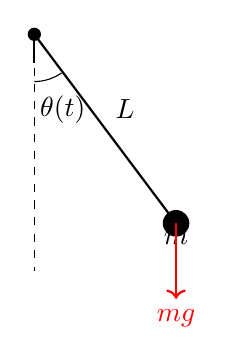
\begin{tikzpicture}[scale=1.2]
        % Pendulum setup
        \draw[thick] (0,0) -- (0,-0.3);
        \fill (0,0) circle (2pt);
        \draw[thick] (0,0) -- (1.5,-2) node[midway,above right] {$L$};
        \fill (1.5,-2) circle (4pt) node[below] {$m$};
        
        % Arc and angle
        \draw[dashed] (0,0) -- (0,-2.5);
        \draw (0,-0.5) arc (-90:-90+35:0.5);
        \node at (0.3,-0.8) {$\theta(t)$};
        
        % Length
        % \draw[<->] (0.2,-0.2) -- (1.3,-1.8) node[midway,above right] {$L$};
        
        % Forces
        \draw[->,red,thick] (1.5,-2) -- (1.5,-2.8) node[below] {$mg$};
      \end{tikzpicture}
      \end{center}
    \end{column}
    \begin{column}{0.7\textwidth}
      \small
      \textbf{Newton: acceleration in tangent direction $a_t$:}
      \begin{align}
        ma_t &= -mg\sin\theta \\
        m L \theta'' &= -mg\sin\theta \\
        \theta'' &= -\frac{g}{L}\sin\theta
      \end{align}
      
      \vspace{0.5em}
      Where:
      \begin{itemize}
        \item $a_t = L\theta''$ (tangential acceleration)
        \item Restoring force: $-mg\sin\theta$
        \item Tension $T$ acts radially (canceled out)
      \end{itemize}
    \end{column}
  \end{columns}
  
  \vspace{0.5em}
  \textbf{Result:} $\theta'' + \frac{g}{L}\sin(\theta) = 0$ (nonlinear due to $\sin\theta$)\\
    % \vspace{0.5em}

  \textbf{Note for small angle $\sin(\theta) \sim \theta$:} $\theta'' + \frac{g}{L} \theta = 0$ and we recover the harmonic oscillator.
\end{frame}
\begin{frame}{Example: nonlinear pendulum}
  \begin{itemize}
    \item The nonlinear pendulum is governed by the ODE
    \[
      \theta''(t) + \frac{g}{L}\sin(\theta(t)) = 0,
    \]
    where $\theta(t)$ is the angle of the pendulum from vertical, $g$ is the acceleration due to gravity, and $L$ is the length of the pendulum.
    \item \textbf{Our code assume first-order ODEs:} We must convert it to a system of first-order ODEs by defining $\omega = \theta'$:
    \[
      \begin{cases}
        \theta' = \omega, \\
        \omega' = -\frac{g}{L}\sin(\theta).
      \end{cases}
    \]
    \item We can now implement this system in our ODE solver class.
  \end{itemize}
\end{frame}

\begin{frame}{What's coming}
\end{frame}
\begin{frame}{This unit's project: 1D helicopter model}
  \begin{center}
    \includegraphics[width=0.9\textwidth]{helicopter.png}
  \end{center}
\end{frame}

\begin{frame}{Wednesday's lab: learn how to use a potentiometer}
  \begin{center}
    \includegraphics[width=0.9\textwidth]{potentiometers.png}
  \end{center}
\end{frame}

\begin{frame}[fragile]{Reading a potentiometer with the picos}
    \small
    \textbf{Goal:} Read analog sensor data using the Raspberry Pi Pico's ADC (analog-to-digital converter)
    
    \begin{columns}
        \begin{column}{0.4\textwidth}
    \begin{minted}[fontsize=\tiny,breaklines=true]{python}
from machine import ADC, Pin
import time

# Initialize ADC on pin 26 (for Raspberry Pi Pico)
potentiometer = ADC(Pin(26))
      
while True:
  # Read the ADC value (0-65535)
    pot_value = potentiometer.read_u16()  
    print("Potentiometer value:", pot_value)
    time.sleep(0.1)
\end{minted}
\end{column}
\begin{column}{0.6\textwidth}
\includegraphics[width=1.0\textwidth]{thonnyPotRead.png}
\end{column}
\end{columns}
\end{frame}

\begin{frame}[fragile]{Getting data off of the pico and onto your laptop to read}
  \textbf{Goal:} Save potentiometer readings to a file on the Pico's filesystem so you can transfer it to your laptop later.
  \vspace{1em}

    \begin{minted}[fontsize=\tiny,breaklines=true]{python}
from machine import ADC, Pin
import time

# Initialize ADC on pin 26 (for Raspberry Pi Pico)
potentiometer = ADC(Pin(26))

# Open the file in write mode
with open("potentiometer_values.txt", "w") as file:
    while True:
        pot_value = potentiometer.read_u16()  # Read the ADC value (0-65535)
        file.write(f"Potentiometer value: {pot_value}\n")
        file.flush()  # Ensure the value is written to the file immediately
        print("Potentiometer value:", pot_value)
        time.sleep(0.1)
\end{minted}
  
  \vspace{0.5em}
  \small
  \textbf{To transfer:} In Thonny, View → Files → Right-click file → Download to computer
\end{frame}

\begin{frame}{Today}
  \begin{itemize}
  \item Step through the pendulum code together
  \item Finish homework together
  \item Get ready for Wednesday's lab
  \item Questions?
  \end{itemize}
\end{frame}
\end{document}
